\documentclass{article}
\usepackage[letterpaper, margin=1in]{geometry}
\usepackage{graphicx}
\usepackage{tcolorbox}
\usepackage{lipsum}
\usepackage{eso-pic}
\usepackage{transparent}
\usepackage{xcolor}
\usepackage{titlesec}
\usepackage{fancyhdr}

% Define colors
\definecolor{titlebg}{RGB}{0,102,204}
\definecolor{leftcol}{RGB}{0,51,102}
\definecolor{titletext}{RGB}{255,255,255}
\definecolor{blacktitle}{RGB}{0,0,0}
\definecolor{codebg}{RGB}{240,240,240} % New color for code background

% Define a new tcolorbox environment for questions without borders
\newtcolorbox{questionbox}{
  colback=white,
  rounded corners,
  boxrule=0pt,
  left=0pt,
  right=0pt,
  top=0pt,
  bottom=0pt,
  before=\vspace{\baselineskip},
  after=\vspace{\baselineskip}
}

% Define a new tcolorbox environment for solutions with curved edges and thicker border
\newtcolorbox{solutionbox}{
  colback=white,
  colframe=black,
  rounded corners,
  boxrule=0.8pt,
  rounded corners=5pt,
  left=0pt,
  right=0pt,
  top=0pt,
  bottom=0pt,
  before=\vspace{\baselineskip},
  after=\vspace{\baselineskip}
}

% Define a new tcolorbox environment for code with rounded corners and background color
\newtcolorbox{codebox}{
  colback=codebg,
  colframe=black,
  rounded corners,
  boxrule=0.8pt,
  left=0pt,
  right=0pt,
  top=0pt,
  bottom=0pt,
  before=\vspace{\baselineskip},
  after=\vspace{\baselineskip}
}

% Customize the title page
\titleformat{\section}[block]{\normalfont\Huge\bfseries\color{blacktitle}}{}{0em}{}[\color{titlebg}\titlerule]

% Customize the section format for question numbers
\titleformat{name=\section,numberless}[block]{\normalfont\Large\bfseries\color{blacktitle}}{}{0em}{}[\color{titlebg}\titlerule]

% Header and Footer settings
\pagestyle{fancy}
\fancyhf{}
\renewcommand{\headrulewidth}{0pt}
\fancyhead[L]{
\includegraphics[width=0.5cm]{images/logo2.png}\hspace{0.5cm}}
\fancyhead[R]{\textbf{Arshia Gharooni}}
\fancyfoot[C]{\thepage}

\begin{document}

% Title Page with Background Image (50% opacity) and Fancy Design
\AddToShipoutPictureBG*{%
  \AtPageLowerLeft{%
    \transparent{0.3}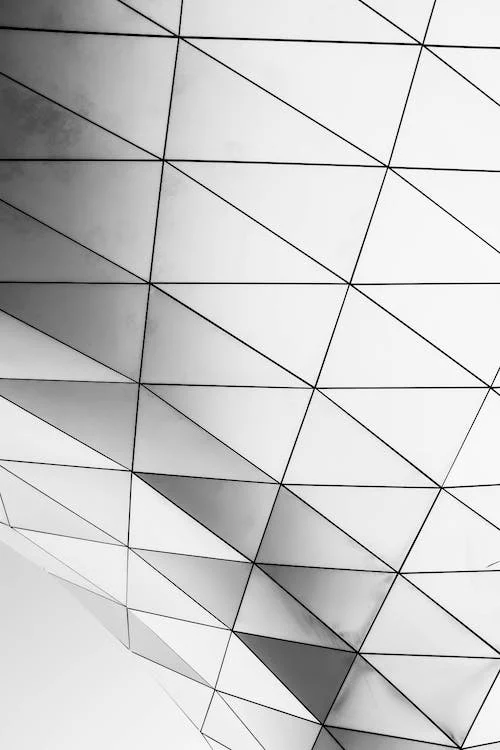
\includegraphics[width=\paperwidth,height=\paperheight]{images/image.png} % Adjust the file name and extension
  }%

  \AtTextLowerLeft{%
    \colorbox{leftcol}{%
      \begin{minipage}{0.3\textwidth}
        \vspace*{1cm}
        \centering
        % Insert your logo here
        
\includegraphics[width=5cm]{images/logo.png}
        \vspace*{1cm}
        
        \textcolor{titletext}{\Large\textbf{January 25}}\par
        \vspace{4cm}
        \textcolor{titletext}{\today}
      \end{minipage}%
    }%
    \hspace{0.05\textwidth} % Adjust the space between columns
    \colorbox{leftcol}{%
      \begin{minipage}{0.6\textwidth}
      \centering
        \vspace*{2cm}
        \textcolor{titletext}{\Huge\textbf{CS234: RL}}\par
        \vspace{1cm}
        \textcolor{titletext}{\Large\textbf{Arshia Gharooni}}
        \vspace{30cm}
      \end{minipage}%
    }%
  }
}

\begin{titlepage}
  \centering
  \vspace*{2cm}
  \textcolor{blacktitle}{}\par
  \vspace{0.5cm}
  \textcolor{blacktitle}{}
\end{titlepage}

\ClearShipoutPictureBG

% Assignment Content
\section*{Question 1}
\begin{questionbox}
What is the capital of France?
\end{questionbox}

\begin{solutionbox}
  The capital of France is Paris.
\end{solutionbox}

\section*{Question 2}
\begin{questionbox}
Solve the equation $2x + 5 = 11$.
\end{questionbox}

\begin{solutionbox}
  The solution to the equation $2x + 5 = 11$ is $x = 3$.
\end{solutionbox}

\section*{Question 3}
\begin{questionbox}
There are 2 cows down there. How many cows are down there?
\end{questionbox}

\begin{solutionbox}
  There are 2 cows down there, and here is the code for it:
\end{solutionbox}

\begin{codebox}
\begin{verbatim}
#include <iostream>

int main() {
    std::cout << "Hello, LaTeX!" << std::endl;
    return 0;
}
\end{verbatim}
\end{codebox}

\section*{Question 4}
\begin{questionbox}
Something Something Something Something Something Something .
\end{questionbox}

\begin{solutionbox}
  Something Something Something Something Something Something.
\end{solutionbox}

\section*{Question 5}
\begin{questionbox}
Something Something Something Something Something Something.
\end{questionbox}

\begin{solutionbox}
  Something Something Something Something Something Something.
\end{solutionbox}

\section*{Question 6}
\begin{questionbox}
Something Something Something Something Something Something.
\end{questionbox}

\begin{solutionbox}
  Research Center for Molecular and Cellular Imaging, Imam Khomeini Hospital Complex, Tehran University of Medical Sciences, Tehran
\end{solutionbox}

% Add more questions, solutions, and code examples as needed

\end{document}
